\documentclass[]{book}
\usepackage{lmodern}
\usepackage{amssymb,amsmath}
\usepackage{ifxetex,ifluatex}
\usepackage{fixltx2e} % provides \textsubscript
\ifnum 0\ifxetex 1\fi\ifluatex 1\fi=0 % if pdftex
  \usepackage[T1]{fontenc}
  \usepackage[utf8]{inputenc}
\else % if luatex or xelatex
  \ifxetex
    \usepackage{mathspec}
  \else
    \usepackage{fontspec}
  \fi
  \defaultfontfeatures{Ligatures=TeX,Scale=MatchLowercase}
\fi
% use upquote if available, for straight quotes in verbatim environments
\IfFileExists{upquote.sty}{\usepackage{upquote}}{}
% use microtype if available
\IfFileExists{microtype.sty}{%
\usepackage{microtype}
\UseMicrotypeSet[protrusion]{basicmath} % disable protrusion for tt fonts
}{}
\usepackage[margin=1in]{geometry}
\usepackage{hyperref}
\hypersetup{unicode=true,
            pdftitle={資料科學與R語言},
            pdfauthor={曾意儒 Yi-Ju Tseng},
            pdfborder={0 0 0},
            breaklinks=true}
\urlstyle{same}  % don't use monospace font for urls
\usepackage{natbib}
\bibliographystyle{apalike}
\usepackage{color}
\usepackage{fancyvrb}
\newcommand{\VerbBar}{|}
\newcommand{\VERB}{\Verb[commandchars=\\\{\}]}
\DefineVerbatimEnvironment{Highlighting}{Verbatim}{commandchars=\\\{\}}
% Add ',fontsize=\small' for more characters per line
\usepackage{framed}
\definecolor{shadecolor}{RGB}{248,248,248}
\newenvironment{Shaded}{\begin{snugshade}}{\end{snugshade}}
\newcommand{\KeywordTok}[1]{\textcolor[rgb]{0.13,0.29,0.53}{\textbf{{#1}}}}
\newcommand{\DataTypeTok}[1]{\textcolor[rgb]{0.13,0.29,0.53}{{#1}}}
\newcommand{\DecValTok}[1]{\textcolor[rgb]{0.00,0.00,0.81}{{#1}}}
\newcommand{\BaseNTok}[1]{\textcolor[rgb]{0.00,0.00,0.81}{{#1}}}
\newcommand{\FloatTok}[1]{\textcolor[rgb]{0.00,0.00,0.81}{{#1}}}
\newcommand{\ConstantTok}[1]{\textcolor[rgb]{0.00,0.00,0.00}{{#1}}}
\newcommand{\CharTok}[1]{\textcolor[rgb]{0.31,0.60,0.02}{{#1}}}
\newcommand{\SpecialCharTok}[1]{\textcolor[rgb]{0.00,0.00,0.00}{{#1}}}
\newcommand{\StringTok}[1]{\textcolor[rgb]{0.31,0.60,0.02}{{#1}}}
\newcommand{\VerbatimStringTok}[1]{\textcolor[rgb]{0.31,0.60,0.02}{{#1}}}
\newcommand{\SpecialStringTok}[1]{\textcolor[rgb]{0.31,0.60,0.02}{{#1}}}
\newcommand{\ImportTok}[1]{{#1}}
\newcommand{\CommentTok}[1]{\textcolor[rgb]{0.56,0.35,0.01}{\textit{{#1}}}}
\newcommand{\DocumentationTok}[1]{\textcolor[rgb]{0.56,0.35,0.01}{\textbf{\textit{{#1}}}}}
\newcommand{\AnnotationTok}[1]{\textcolor[rgb]{0.56,0.35,0.01}{\textbf{\textit{{#1}}}}}
\newcommand{\CommentVarTok}[1]{\textcolor[rgb]{0.56,0.35,0.01}{\textbf{\textit{{#1}}}}}
\newcommand{\OtherTok}[1]{\textcolor[rgb]{0.56,0.35,0.01}{{#1}}}
\newcommand{\FunctionTok}[1]{\textcolor[rgb]{0.00,0.00,0.00}{{#1}}}
\newcommand{\VariableTok}[1]{\textcolor[rgb]{0.00,0.00,0.00}{{#1}}}
\newcommand{\ControlFlowTok}[1]{\textcolor[rgb]{0.13,0.29,0.53}{\textbf{{#1}}}}
\newcommand{\OperatorTok}[1]{\textcolor[rgb]{0.81,0.36,0.00}{\textbf{{#1}}}}
\newcommand{\BuiltInTok}[1]{{#1}}
\newcommand{\ExtensionTok}[1]{{#1}}
\newcommand{\PreprocessorTok}[1]{\textcolor[rgb]{0.56,0.35,0.01}{\textit{{#1}}}}
\newcommand{\AttributeTok}[1]{\textcolor[rgb]{0.77,0.63,0.00}{{#1}}}
\newcommand{\RegionMarkerTok}[1]{{#1}}
\newcommand{\InformationTok}[1]{\textcolor[rgb]{0.56,0.35,0.01}{\textbf{\textit{{#1}}}}}
\newcommand{\WarningTok}[1]{\textcolor[rgb]{0.56,0.35,0.01}{\textbf{\textit{{#1}}}}}
\newcommand{\AlertTok}[1]{\textcolor[rgb]{0.94,0.16,0.16}{{#1}}}
\newcommand{\ErrorTok}[1]{\textcolor[rgb]{0.64,0.00,0.00}{\textbf{{#1}}}}
\newcommand{\NormalTok}[1]{{#1}}
\usepackage{longtable,booktabs}
\usepackage{graphicx,grffile}
\makeatletter
\def\maxwidth{\ifdim\Gin@nat@width>\linewidth\linewidth\else\Gin@nat@width\fi}
\def\maxheight{\ifdim\Gin@nat@height>\textheight\textheight\else\Gin@nat@height\fi}
\makeatother
% Scale images if necessary, so that they will not overflow the page
% margins by default, and it is still possible to overwrite the defaults
% using explicit options in \includegraphics[width, height, ...]{}
\setkeys{Gin}{width=\maxwidth,height=\maxheight,keepaspectratio}
\IfFileExists{parskip.sty}{%
\usepackage{parskip}
}{% else
\setlength{\parindent}{0pt}
\setlength{\parskip}{6pt plus 2pt minus 1pt}
}
\setlength{\emergencystretch}{3em}  % prevent overfull lines
\providecommand{\tightlist}{%
  \setlength{\itemsep}{0pt}\setlength{\parskip}{0pt}}
\setcounter{secnumdepth}{5}
% Redefines (sub)paragraphs to behave more like sections
\ifx\paragraph\undefined\else
\let\oldparagraph\paragraph
\renewcommand{\paragraph}[1]{\oldparagraph{#1}\mbox{}}
\fi
\ifx\subparagraph\undefined\else
\let\oldsubparagraph\subparagraph
\renewcommand{\subparagraph}[1]{\oldsubparagraph{#1}\mbox{}}
\fi

%%% Use protect on footnotes to avoid problems with footnotes in titles
\let\rmarkdownfootnote\footnote%
\def\footnote{\protect\rmarkdownfootnote}

%%% Change title format to be more compact
\usepackage{titling}

% Create subtitle command for use in maketitle
\newcommand{\subtitle}[1]{
  \posttitle{
    \begin{center}\large#1\end{center}
    }
}

\setlength{\droptitle}{-2em}
  \title{資料科學與R語言}
  \pretitle{\vspace{\droptitle}\centering\huge}
  \posttitle{\par}
  \author{曾意儒 Yi-Ju Tseng}
  \preauthor{\centering\large\emph}
  \postauthor{\par}
  \predate{\centering\large\emph}
  \postdate{\par}
  \date{2017-02-06}

\usepackage{booktabs}
\usepackage{amsthm}

\usepackage{CJKutf8}

\makeatletter
\def\thm@space@setup{%
  \thm@preskip=8pt plus 2pt minus 4pt
  \thm@postskip=\thm@preskip
}
\makeatother

\usepackage{amsthm}
\newtheorem{theorem}{Theorem}[chapter]
\newtheorem{lemma}{Lemma}[chapter]
\theoremstyle{definition}
\newtheorem{definition}{Definition}[chapter]
\newtheorem{corollary}{Corollary}[chapter]
\newtheorem{proposition}{Proposition}[chapter]
\theoremstyle{definition}
\newtheorem{example}{Example}[chapter]
\theoremstyle{remark}
\newtheorem*{remark}{Remark}
\begin{document}
\maketitle

{
\setcounter{tocdepth}{1}
\tableofcontents
}
\chapter*{}\label{preface}
\addcontentsline{toc}{chapter}{}

長庚大學資訊管理學系大數據分析方法教學使用書籍,內容包括使用M語言做資料擷取、資料清洗與處理、探索式資料分析、資料視覺化與資料探勘等,並介紹R與Hadoop
EcoSystems介接方法。

\chapter{R語言101}\label{intro}

本章節介紹基本的R語言,包括基本指令操作、運算子介紹。

\section{什麼是R語言}\label{r}

\href{http://www.r-project.org/}{R語言}是一種自由軟體程式語言,主要用於資料分析與統計運算,其發展歷史可參考\href{https://zh.wikipedia.org/wiki/R\%E8\%AF\%AD\%E8\%A8\%80}{維基百科}。基本的R軟體已經內建多種統計學及數字分析功能,其餘功能可以透過安裝\textbf{套件(Packages)}加載,截至2017年1月為止,R軟體可另外安裝的套件數目共有10,000個以上
(\href{https://www.rstudio.com/rviews/2017/01/06/10000-cran-packages/}{R
Studio報導})。常用的套件清單可參考各項網路資訊,如\href{https://support.rstudio.com/hc/en-us/articles/201057987-Quick-list-of-useful-R-packages}{R
Studio的整理:Quick list of useful R packages}

安裝套件Package的方法如下:

\begin{Shaded}
\begin{Highlighting}[]
\KeywordTok{install.packages}\NormalTok{(}\StringTok{"套件名稱"}\NormalTok{)}
\end{Highlighting}
\end{Shaded}

值得注意的是,套件名稱需要加上雙引號,舉例來說,若要安裝\texttt{ggplot2}套件,則要在R的Console視窗內輸入:

\begin{Shaded}
\begin{Highlighting}[]
\KeywordTok{install.packages}\NormalTok{(}\StringTok{"ggplot2"}\NormalTok{)}
\end{Highlighting}
\end{Shaded}

若要載入\textbf{已安裝}的套件,則輸入\texttt{library(套件名稱)},範例:

\begin{Shaded}
\begin{Highlighting}[]
\KeywordTok{library}\NormalTok{(ggplot2)}
\end{Highlighting}
\end{Shaded}

載入已安裝的套件時,不用再套件名稱前後加雙引號。

\section{變數設定}

在開始深入學習R語言之前,首要任務是學習最基本的R程式碼:\textbf{變數設定},在R語言中,主要使用\texttt{\textless{}-}設定變數,設定方法為:\textbf{變數名稱}\texttt{\textless{}-}\textbf{變數內容},雖然\textbf{變數名稱}可依箭頭方向放置於左側\texttt{\textless{}-}或右側\texttt{-\textgreater{}},但為方便閱讀,\textbf{變數名稱}多放置於左側。

\begin{Shaded}
\begin{Highlighting}[]
\NormalTok{a<-}\DecValTok{1} 
\DecValTok{2}\NormalTok{->b}
\NormalTok{a}
\end{Highlighting}
\end{Shaded}

\begin{verbatim}
## [1] 1
\end{verbatim}

\begin{Shaded}
\begin{Highlighting}[]
\NormalTok{b}
\end{Highlighting}
\end{Shaded}

\begin{verbatim}
## [1] 2
\end{verbatim}

R語言也接受使用\texttt{=}設定變數,此時\textbf{變數名稱}必須在左側,如:\textbf{變數名稱}\texttt{=}\textbf{變數內容}

\begin{Shaded}
\begin{Highlighting}[]
\NormalTok{c=}\DecValTok{1} 
\NormalTok{c}
\end{Highlighting}
\end{Shaded}

\begin{verbatim}
## [1] 1
\end{verbatim}

除了\textbf{變數設定}外,\texttt{str()}函數也為常用基本函數,\texttt{str()}用在檢查與總覽各類變數型態。

\begin{Shaded}
\begin{Highlighting}[]
\NormalTok{d<-}\DecValTok{3}
\KeywordTok{str}\NormalTok{(d)}
\end{Highlighting}
\end{Shaded}

\begin{verbatim}
##  num 3
\end{verbatim}

\section{資料型態}

在R語言中,常用的資料型態包括\textbf{數值 (numeric)}、\textbf{字串
(character)}、\textbf{布林變數 (logic)}以及\textbf{日期 (Date)}等。

\subsection{數值 numeric}\label{-numeric}

數值包括整數(沒有小數點)與符點數(有小數點)的數值

\begin{Shaded}
\begin{Highlighting}[]
\NormalTok{num1<-}\DecValTok{100} 
\NormalTok{num2<-}\FloatTok{1000.001}
\end{Highlighting}
\end{Shaded}

值得注意的是,若數值長度超過 \texttt{2\^{}53},必須導入\texttt{bit64}
package
\citep{R-bit64},將數值長度上限提高為\texttt{2\^{}63},才能表示完整數值

\begin{Shaded}
\begin{Highlighting}[]
\KeywordTok{print}\NormalTok{(}\DecValTok{2}\NormalTok{^}\DecValTok{53}\NormalTok{, }\DataTypeTok{digits=}\DecValTok{20}\NormalTok{) }
\end{Highlighting}
\end{Shaded}

\begin{verbatim}
## [1] 9007199254740992
\end{verbatim}

\begin{Shaded}
\begin{Highlighting}[]
\KeywordTok{print}\NormalTok{(}\DecValTok{2}\NormalTok{^}\DecValTok{53+1}\NormalTok{, }\DataTypeTok{digits=}\DecValTok{20}\NormalTok{) }\CommentTok{# +1後,數值仍與2^53相同}
\end{Highlighting}
\end{Shaded}

\begin{verbatim}
## [1] 9007199254740992
\end{verbatim}

\begin{Shaded}
\begin{Highlighting}[]
\KeywordTok{library}\NormalTok{(bit64) }\CommentTok{# 導入bit64 package}
\KeywordTok{print}\NormalTok{(}\KeywordTok{as.integer64}\NormalTok{(}\DecValTok{2}\NormalTok{)^}\DecValTok{53}\NormalTok{, }\DataTypeTok{digits=}\DecValTok{20}\NormalTok{)}
\end{Highlighting}
\end{Shaded}

\begin{verbatim}
## integer64
## [1] 9007199254740992
\end{verbatim}

\begin{Shaded}
\begin{Highlighting}[]
\KeywordTok{print}\NormalTok{(}\KeywordTok{as.integer64}\NormalTok{(}\DecValTok{2}\NormalTok{)^}\DecValTok{53+1}\NormalTok{, }\DataTypeTok{digits=}\DecValTok{20}\NormalTok{)}\CommentTok{# 導入bit64後,可得正確答案}
\end{Highlighting}
\end{Shaded}

\begin{verbatim}
## integer64
## [1] 9007199254740993
\end{verbatim}

\subsection{字串 character}\label{-character}

用雙引號\texttt{"}框起的文字會被儲存為字串格式,若在數字前後加上雙引號,數字也會被儲存為文字形式,無法進行數值的加減乘除等運算。

\begin{Shaded}
\begin{Highlighting}[]
\NormalTok{char1<-}\StringTok{"abcTest"} 
\NormalTok{char2<-}\StringTok{"100"}
\NormalTok{char3<-}\StringTok{"200"}
\CommentTok{#char2+char3 #會輸出Error message: non-numeric argument to binary operator}
\end{Highlighting}
\end{Shaded}

\subsection{布林變數 logic}\label{-logic}

用於邏輯判斷,可使用大寫\textbf{TRUE}或\textbf{T}代表\textbf{真},大寫\textbf{FALSE}或\textbf{F}代表假。

\begin{Shaded}
\begin{Highlighting}[]
\NormalTok{boolT<-}\OtherTok{TRUE}
\NormalTok{boolT1<-T}
\NormalTok{boolF<-}\OtherTok{FALSE}
\NormalTok{boolF1<-F}
\end{Highlighting}
\end{Shaded}

\subsection{日期 (Date)}\label{-date}

用於表示日期,於資料分析中常用,使用\texttt{Sys.Date()}指定可得系統日期。

\begin{Shaded}
\begin{Highlighting}[]
\NormalTok{dateBook<-}\KeywordTok{Sys.Date}\NormalTok{()}
\NormalTok{dateBook}
\end{Highlighting}
\end{Shaded}

\begin{verbatim}
## [1] "2017-02-06"
\end{verbatim}

日期與字串的相關轉換操作可考慮使用簡單易懂的\texttt{lubridate}\citep{R-lubridate}
package,如果想要將\texttt{年/月/日}格式的文字轉換為日期物件,可使用\texttt{ymd()}函數(y表年year,m表月month,d表日day),如果想要將\texttt{月/日/年}格式的文字轉換為日期物件,則使用\texttt{mdy()}函數,以此類推。

\begin{Shaded}
\begin{Highlighting}[]
\KeywordTok{library}\NormalTok{(lubridate)}
\KeywordTok{ymd}\NormalTok{(}\StringTok{'2012/3/3'}\NormalTok{)}
\end{Highlighting}
\end{Shaded}

\begin{verbatim}
## [1] "2012-03-03"
\end{verbatim}

\begin{Shaded}
\begin{Highlighting}[]
\KeywordTok{mdy}\NormalTok{(}\StringTok{'3/3/2012'}\NormalTok{)}
\end{Highlighting}
\end{Shaded}

\begin{verbatim}
## [1] "2012-03-03"
\end{verbatim}

其他使用方式可參考
\href{http://blog.yhat.com/static/pdf/R_date_cheat_sheet.pdf}{The Yhat
Blog}。

\section{基本運算子}

\subsection{數學運算}

在R中,數學運算與其他程式語言相同

\begin{itemize}
\tightlist
\item
  加 \texttt{+}
\item
  減 \texttt{-}
\item
  乘 \texttt{*}
\item
  除 \texttt{/}
\end{itemize}

\begin{Shaded}
\begin{Highlighting}[]
\NormalTok{num1<-}\DecValTok{1}
\NormalTok{num2<-}\DecValTok{100}
\NormalTok{num1+num2}
\end{Highlighting}
\end{Shaded}

\begin{verbatim}
## [1] 101
\end{verbatim}

\begin{Shaded}
\begin{Highlighting}[]
\NormalTok{num1-num2}
\end{Highlighting}
\end{Shaded}

\begin{verbatim}
## [1] -99
\end{verbatim}

\begin{Shaded}
\begin{Highlighting}[]
\NormalTok{num1*num2}
\end{Highlighting}
\end{Shaded}

\begin{verbatim}
## [1] 100
\end{verbatim}

\begin{Shaded}
\begin{Highlighting}[]
\NormalTok{num1/num2}
\end{Highlighting}
\end{Shaded}

\begin{verbatim}
## [1] 0.01
\end{verbatim}

\subsection{邏輯運算}

常用之邏輯判斷也可在R中直接使用

\begin{itemize}
\tightlist
\item
  大於 \texttt{\textgreater{}}
\item
  小於 \texttt{\textless{}}
\item
  等於
  \texttt{==},為了不與變數設定混淆,判斷兩遍數是否相等,要用\textbf{雙等號}
\item
  大於等於 \texttt{\textgreater{}=}
\item
  小於等於 \texttt{\textless{}=}
\end{itemize}

\begin{Shaded}
\begin{Highlighting}[]
\NormalTok{num1<-}\DecValTok{1}
\NormalTok{num2<-}\DecValTok{100}
\NormalTok{num1>num2}
\end{Highlighting}
\end{Shaded}

\begin{verbatim}
## [1] FALSE
\end{verbatim}

\begin{Shaded}
\begin{Highlighting}[]
\NormalTok{num1<num2}
\end{Highlighting}
\end{Shaded}

\begin{verbatim}
## [1] TRUE
\end{verbatim}

文字字串也可比較大小

\begin{Shaded}
\begin{Highlighting}[]
\NormalTok{char1<-}\StringTok{"abcTest"} 
\NormalTok{char2<-}\StringTok{"defTest"}
\NormalTok{char1>char2}
\end{Highlighting}
\end{Shaded}

\begin{verbatim}
## [1] FALSE
\end{verbatim}

邏輯混合判斷,和JAVA等語言不同的是,在R中使用\textbf{單符號}即可表示且\texttt{\&}和或\texttt{\textbar{}}

\begin{itemize}
\tightlist
\item
  且 \texttt{\&}
\item
  或 \texttt{\textbar{}}
\end{itemize}

\begin{Shaded}
\begin{Highlighting}[]
\OtherTok{TRUE} \NormalTok{&}\StringTok{ }\OtherTok{TRUE}
\end{Highlighting}
\end{Shaded}

\begin{verbatim}
## [1] TRUE
\end{verbatim}

\begin{Shaded}
\begin{Highlighting}[]
\OtherTok{TRUE} \NormalTok{&}\StringTok{ }\OtherTok{FALSE}
\end{Highlighting}
\end{Shaded}

\begin{verbatim}
## [1] FALSE
\end{verbatim}

\begin{Shaded}
\begin{Highlighting}[]
\OtherTok{TRUE} \NormalTok{|}\StringTok{ }\OtherTok{TRUE}
\end{Highlighting}
\end{Shaded}

\begin{verbatim}
## [1] TRUE
\end{verbatim}

\begin{Shaded}
\begin{Highlighting}[]
\OtherTok{TRUE} \NormalTok{|}\StringTok{ }\OtherTok{FALSE}
\end{Highlighting}
\end{Shaded}

\begin{verbatim}
## [1] TRUE
\end{verbatim}

\section{rbookdown原始範例,暫留}\label{rbookdown}

You can label chapter and section titles using \texttt{\{\#label\}}
after them, e.g., we can reference Chapter \ref{intro}. If you do not
manually label them, there will be automatic labels anyway, e.g.,
Chapter \ref{methods}.

Figures and tables with captions will be placed in \texttt{figure} and
\texttt{table} environments, respectively.

\begin{Shaded}
\begin{Highlighting}[]
\KeywordTok{par}\NormalTok{(}\DataTypeTok{mar =} \KeywordTok{c}\NormalTok{(}\DecValTok{4}\NormalTok{, }\DecValTok{4}\NormalTok{, .}\DecValTok{1}\NormalTok{, .}\DecValTok{1}\NormalTok{))}
\KeywordTok{plot}\NormalTok{(pressure, }\DataTypeTok{type =} \StringTok{'b'}\NormalTok{, }\DataTypeTok{pch =} \DecValTok{19}\NormalTok{)}
\end{Highlighting}
\end{Shaded}

\begin{figure}

{\centering 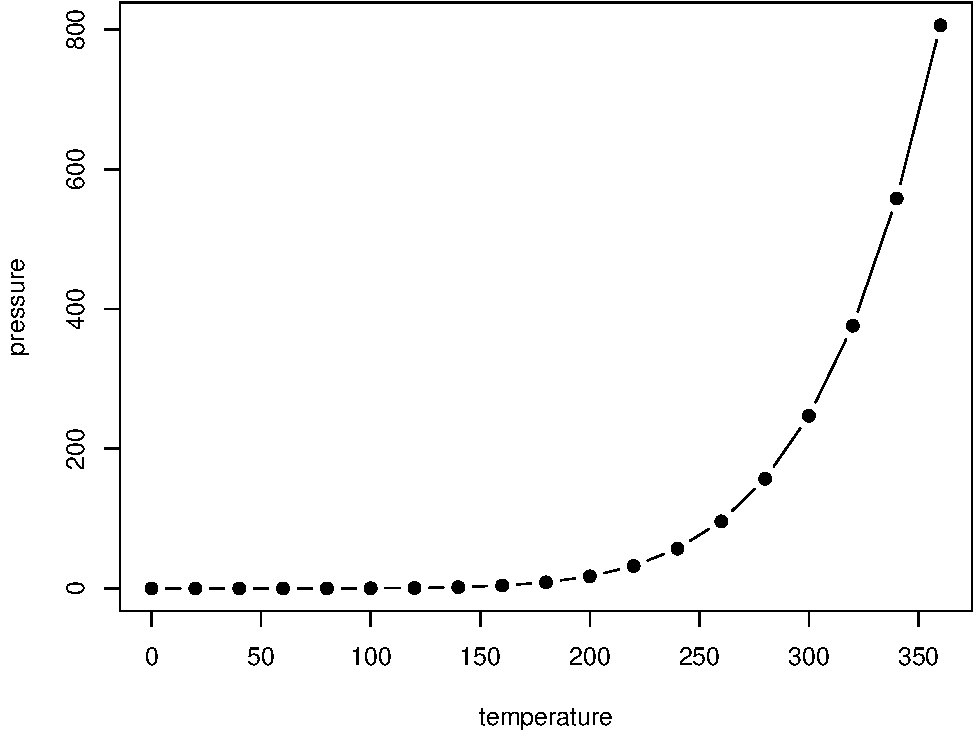
\includegraphics[width=0.8\linewidth]{DataAnalyticsWithR_files/figure-latex/nice-fig-1} 

}

\caption{Here is a nice figure!}\label{fig:nice-fig}
\end{figure}

Reference a figure by its code chunk label with the \texttt{fig:}
prefix, e.g., see Figure \ref{fig:nice-fig}. Similarly, you can
reference tables generated from \texttt{knitr::kable()}, e.g., see Table
\ref{tab:nice-tab}.

\begin{Shaded}
\begin{Highlighting}[]
\NormalTok{knitr::}\KeywordTok{kable}\NormalTok{(}
  \KeywordTok{head}\NormalTok{(iris, }\DecValTok{20}\NormalTok{), }\DataTypeTok{caption =} \StringTok{'Here is a nice table!'}\NormalTok{,}
  \DataTypeTok{booktabs =} \OtherTok{TRUE}
\NormalTok{)}
\end{Highlighting}
\end{Shaded}

\begin{table}

\caption{\label{tab:nice-tab}Here is a nice table!}
\centering
\begin{tabular}[t]{rrrrl}
\toprule
Sepal.Length & Sepal.Width & Petal.Length & Petal.Width & Species\\
\midrule
5.1 & 3.5 & 1.4 & 0.2 & setosa\\
4.9 & 3.0 & 1.4 & 0.2 & setosa\\
4.7 & 3.2 & 1.3 & 0.2 & setosa\\
4.6 & 3.1 & 1.5 & 0.2 & setosa\\
5.0 & 3.6 & 1.4 & 0.2 & setosa\\
\addlinespace
5.4 & 3.9 & 1.7 & 0.4 & setosa\\
4.6 & 3.4 & 1.4 & 0.3 & setosa\\
5.0 & 3.4 & 1.5 & 0.2 & setosa\\
4.4 & 2.9 & 1.4 & 0.2 & setosa\\
4.9 & 3.1 & 1.5 & 0.1 & setosa\\
\addlinespace
5.4 & 3.7 & 1.5 & 0.2 & setosa\\
4.8 & 3.4 & 1.6 & 0.2 & setosa\\
4.8 & 3.0 & 1.4 & 0.1 & setosa\\
4.3 & 3.0 & 1.1 & 0.1 & setosa\\
5.8 & 4.0 & 1.2 & 0.2 & setosa\\
\addlinespace
5.7 & 4.4 & 1.5 & 0.4 & setosa\\
5.4 & 3.9 & 1.3 & 0.4 & setosa\\
5.1 & 3.5 & 1.4 & 0.3 & setosa\\
5.7 & 3.8 & 1.7 & 0.3 & setosa\\
5.1 & 3.8 & 1.5 & 0.3 & setosa\\
\bottomrule
\end{tabular}
\end{table}

You can write citations, too. For example, we are using the
\textbf{bookdown} package \citep{R-bookdown} in this sample book, which
was built on top of R Markdown and \textbf{knitr} \citep{xie2015}.

\chapter{R 資料結構}\label{RDataStructure}

Here is a review of existing methods. \textbf{因子 (factor)}、

\section{向量 vector}\label{-vector}

向量為一維資料的表現和儲存方式,用\texttt{c()}函數可定義向量,如:

\begin{Shaded}
\begin{Highlighting}[]
\NormalTok{vec<-}\KeywordTok{c}\NormalTok{(}\StringTok{'a'}\NormalTok{,}\StringTok{'b'}\NormalTok{,}\StringTok{'c'}\NormalTok{,}\StringTok{'d'}\NormalTok{,}\StringTok{'e'}\NormalTok{)}
\NormalTok{vec}
\end{Highlighting}
\end{Shaded}

\begin{verbatim}
## [1] "a" "b" "c" "d" "e"
\end{verbatim}

a\textasciitilde{}e為vec向量中的\textbf{元素(element)},各元素向中的順序固定,\texttt{a}為\texttt{vec}向量中的第\textbf{1}個元素,\texttt{b}則為第\textbf{2}個元素,以此類推,若要將\texttt{vec}向量的第\textbf{4}個元素取出,可使用

\begin{Shaded}
\begin{Highlighting}[]
\NormalTok{vec[}\DecValTok{4}\NormalTok{] ## 第4個元素}
\end{Highlighting}
\end{Shaded}

\begin{verbatim}
## [1] "d"
\end{verbatim}

此外,在同一向量中,所有元素之\textbf{資料型態必須相同},如上述\texttt{vec}向量,元素均為文字型態。

\subsection{快速產生向量函數}

\subsection{向量運算}

\section{因子 factor}\label{-factor}

\begin{Shaded}
\begin{Highlighting}[]
\NormalTok{char1<-}\StringTok{"abcTest"} 
\NormalTok{char2<-}\StringTok{"100"}
\NormalTok{char3<-}\StringTok{"200"}
\CommentTok{#char2+char3 #會輸出Error message: non-numeric argument to binary operator}
\end{Highlighting}
\end{Shaded}

\section{列表 list}\label{-list}

\section{矩陣 matrix}\label{-matrix}

\section{資料框 data.frame}\label{-data.frame}

\section{資料表 data.table (快)}\label{-data.table-}

\chapter{資料讀取與匯出}\label{io}

What is `Data'?

\url{http://en.wikipedia.org/wiki/Data}

\texttt{Data\ are\ values\ of\ qualitative\ or\ quantitative\ variables,\ belonging\ to\ a\ set\ of\ items.}

看完本章會學到:

\begin{itemize}
\tightlist
\item
  找資料、抓資料、總之就是弄到資料
\item
  資料前處理原則:tidy
\item
  用R做到以上工作
\end{itemize}

\texttt{Raw\ data} -\textgreater{} \textbf{Processing script}
-\textgreater{} \texttt{Tidy\ data} -\textgreater{} Data analysis
-\textgreater{} Data communication

\section{資料類型}

\subsection{Tidy Data}\label{tidy-data}

\begin{itemize}
\tightlist
\item
  一個欄位(Column)內只有一個數值,最好要有凡人看得懂的Column Name
\item
  不同的觀察值應該要在不同行(Raw)
\item
  一張表裡面,有所有分析需要的資料
\item
  如果一定要多張表,中間一定要有index可以把表串起來
\item
  One file, one table
\end{itemize}

\begin{Shaded}
\begin{Highlighting}[]
\NormalTok{if (!}\KeywordTok{require}\NormalTok{(}\StringTok{'SportsAnalytics'}\NormalTok{))\{}
    \KeywordTok{install.packages}\NormalTok{(}\StringTok{"SportsAnalytics"}\NormalTok{)}
    \KeywordTok{library}\NormalTok{(SportsAnalytics)}
\NormalTok{\}}
\NormalTok{NBA1415<-}\KeywordTok{fetch_NBAPlayerStatistics}\NormalTok{(}\StringTok{"14-15"}\NormalTok{)}
\end{Highlighting}
\end{Shaded}

\begin{Shaded}
\begin{Highlighting}[]
\KeywordTok{head}\NormalTok{(NBA1415)}
\end{Highlighting}
\end{Shaded}

\begin{verbatim}
##   League          Name Team Position GamesPlayed
## 1    NBA    Quincy Acy  NYK       SF          68
## 2    NBA  Jordan Adams  MEM       SG          30
## 3    NBA  Steven Adams  OKL        C          70
## 4    NBA   Jeff Adrien  MIN       PF          17
## 5    NBA Arron Afflalo  POR       SG          78
## 6    NBA Alexis Ajinca  NOR        C          68
##   TotalMinutesPlayed FieldGoalsMade
## 1               1288            152
## 2                249             35
## 3               1776            217
## 4                215             19
## 5               2502            375
## 6                956            181
##   FieldGoalsAttempted ThreesMade ThreesAttempted
## 1                 331         18              60
## 2                  86         10              25
## 3                 399          0               2
## 4                  44          0               0
## 5                 884        118             333
## 6                 328          0               0
##   FreeThrowsMade FreeThrowsAttempted OffensiveRebounds
## 1             76                  97                79
## 2             14                  23                 9
## 3            103                 205               199
## 4             22                  38                23
## 5            167                 198                27
## 6             81                  99               104
##   TotalRebounds Assists Steals Turnovers Blocks
## 1           301      68     27        60     22
## 2            28      16     16        14      7
## 3           522      65     38        99     85
## 4            77      15      4         9      9
## 5           247     129     41       116      7
## 6           315      47     21        69     51
##   PersonalFouls Disqualifications TotalPoints
## 1           147                 1         398
## 2            24                 0          94
## 3           222                 3         537
## 4            30                 0          60
## 5           167                 1        1035
## 6           151                 0         443
##   Technicals Ejections FlagrantFouls GamesStarted
## 1          5         0             0           22
## 2          0         0             0            0
## 3          3         0             0           67
## 4          0         0             0            0
## 5          0         0             0           72
## 6          1         0             0            8
\end{verbatim}

\subsection{真實世界裡的Raw Data}\label{raw-data}

\subsubsection{Html}\label{html}

\subsubsection{Facebook}\label{facebook}

\subsubsection{!?}\label{section}

\section{資料到底在哪裡?}

\begin{itemize}
\tightlist
\item
  硬碟裡
\item
  網路下載
\item
  Open Data

  \begin{itemize}
  \tightlist
  \item
    \url{http://data.taipei/}
  \item
    \url{http://data.tycg.gov.tw/}
  \item
    \url{http://data.moi.gov.tw/}
  \end{itemize}
\item
  網頁裡(爬蟲!)
\item
  任何地方
\end{itemize}

\subsection{Open Data}\label{open-data}

\url{http://bit.ly/1U3pVoI}

\section{讀取各類檔案}

\subsection{表格(.csv / Tab分隔 / Excel)}\label{.csv-tab-excel}

\texttt{read.table}, \texttt{read.csv}, 讀取表格資料

The \texttt{read.table}, \texttt{read.csv} 是最常見的,會用這些就好

有以下參數:

\begin{itemize}
\tightlist
\item
  \texttt{file}, 檔名
\item
  \texttt{header}, 是否有欄位名稱(表頭)(T/F)
\item
  \texttt{sep}, 分隔符號
\item
  \texttt{colClasses}, 每一個欄位的類別,用向量表示
\item
  \texttt{comment.char}, 把欄位包起來的符號
\item
  \texttt{skip}, 要跳過幾行?
\item
  \texttt{stringsAsFactors}, 要不要輸入成'Factor'(有序因子)
\end{itemize}

要安裝xlsx 套件

\begin{Shaded}
\begin{Highlighting}[]
\NormalTok{if (!}\KeywordTok{require}\NormalTok{(}\StringTok{'xlsx'}\NormalTok{))\{}
    \KeywordTok{install.packages}\NormalTok{(}\StringTok{"xlsx"}\NormalTok{)}
    \KeywordTok{library}\NormalTok{(xlsx)}
\NormalTok{\}}
\NormalTok{ExcelData <-}\StringTok{ }\KeywordTok{read.xlsx}\NormalTok{(}\StringTok{"data.xlsx"}\NormalTok{,}\DataTypeTok{sheetIndex=}\DecValTok{1}\NormalTok{,}\DataTypeTok{header=}\OtherTok{TRUE}\NormalTok{)}
\KeywordTok{head}\NormalTok{(ExcelData)}
\end{Highlighting}
\end{Shaded}

\section{read.csv使用範例}\label{read.csv}

完全不用給參數

\begin{Shaded}
\begin{Highlighting}[]
\NormalTok{data <-}\StringTok{ }\KeywordTok{read.csv}\NormalTok{(}\StringTok{'open.csv'}\NormalTok{)}
\NormalTok{data}
\end{Highlighting}
\end{Shaded}

\subsection{文字資料}

\texttt{readLines}, 逐行讀取文字資料

\subsection{R檔案格式}\label{r}

\texttt{load}, 讀取已經在R裡面的資料(Ex: iris)

\subsection{R程式}\label{r}

\texttt{source}, 讀R的Obejct or script, 執行, ASCII
(\texttt{dump}的相反)

\section{各類檔案匯出}

寫檔的函數跟讀檔很像:

\subsection{表格(.csv / Tab分隔)}\label{.csv-tab}

\texttt{write.table}

\subsection{文字資料}\label{-1}

\texttt{writeLines}

\subsection{R檔案格式}\label{r-1}

\texttt{save}

\subsection{R程式}\label{r-1}

\texttt{dump}

\section{讀檔的時候R會自動}\label{r}

\begin{itemize}
\tightlist
\item
  跳過\#開頭的任何行(Row)
\item
  判斷要讀幾行
\item
  判斷每個列(Column)的類別
\item
  把欄位包起來的符號
\end{itemize}

如果讀取時已指定\textbf{Column類別}以及\textbf{把欄位包起來的符號},會快很多

\begin{Shaded}
\begin{Highlighting}[]
\NormalTok{initial <-}\StringTok{ }\KeywordTok{read.csv}\NormalTok{(}\StringTok{"open.csv"}\NormalTok{, }\DataTypeTok{nrows =} \DecValTok{100}\NormalTok{)}
\NormalTok{classes <-}\StringTok{ }\KeywordTok{sapply}\NormalTok{(initial, class)}
\NormalTok{tabAll <-}\StringTok{ }\KeywordTok{read.csv}\NormalTok{(}\StringTok{"open.csv"}\NormalTok{, }\DataTypeTok{colClasses =} \NormalTok{classes)}
\end{Highlighting}
\end{Shaded}

\section{從網路上下載檔案 download.file}\label{-download.file}

使用RCurl Package

download.file(URL, destfile=儲存檔名, method=?)

method = ``curl''--\textgreater{}For \textbf{https}

\begin{Shaded}
\begin{Highlighting}[]
\NormalTok{if (!}\KeywordTok{require}\NormalTok{(}\StringTok{'RCurl'}\NormalTok{))\{}
    \KeywordTok{install.packages}\NormalTok{(}\StringTok{"RCurl"}\NormalTok{)}
    \KeywordTok{library}\NormalTok{(RCurl)}
\NormalTok{\}}
\KeywordTok{download.file}\NormalTok{(}\StringTok{"https://raw.githubusercontent.com/yijutseng/BigDataCGUIM/master/files/opendata10401.csv"}\NormalTok{, }
              \DataTypeTok{destfile =} \StringTok{"open.csv"}\NormalTok{, }\DataTypeTok{method =} \StringTok{"curl"}\NormalTok{)}
\end{Highlighting}
\end{Shaded}

\section{Open Data}\label{open-data-1}

\section{爬蟲}

\chapter{資料處理與清洗}\label{manipulation}

Some \emph{significant} applications are demonstrated in this chapter.

\section{Example one}\label{example-one}

\section{Example two}\label{example-two}

\chapter{控制流程}\label{controlstructure}

\section{條件判斷}

\subsection{if-else敘述}\label{if-else}

\textbf{if-else}敘述使用在邏輯判斷,若需要依條件改變需要執行的程式碼,就會使用\textbf{if-else},若\textbf{if}後所接邏輯判斷為\textbf{真(TRUE)},就會執行if下方之程式碼,若為\textbf{偽(FALSE)},則執行\textbf{else}下方之程式碼,若程式中沒有\textbf{else}片段,則不執行任何程式碼。

\begin{Shaded}
\begin{Highlighting}[]
\NormalTok{knitr::}\KeywordTok{include_graphics}\NormalTok{(}\StringTok{"figure/ifelse.png"}\NormalTok{)}
\end{Highlighting}
\end{Shaded}

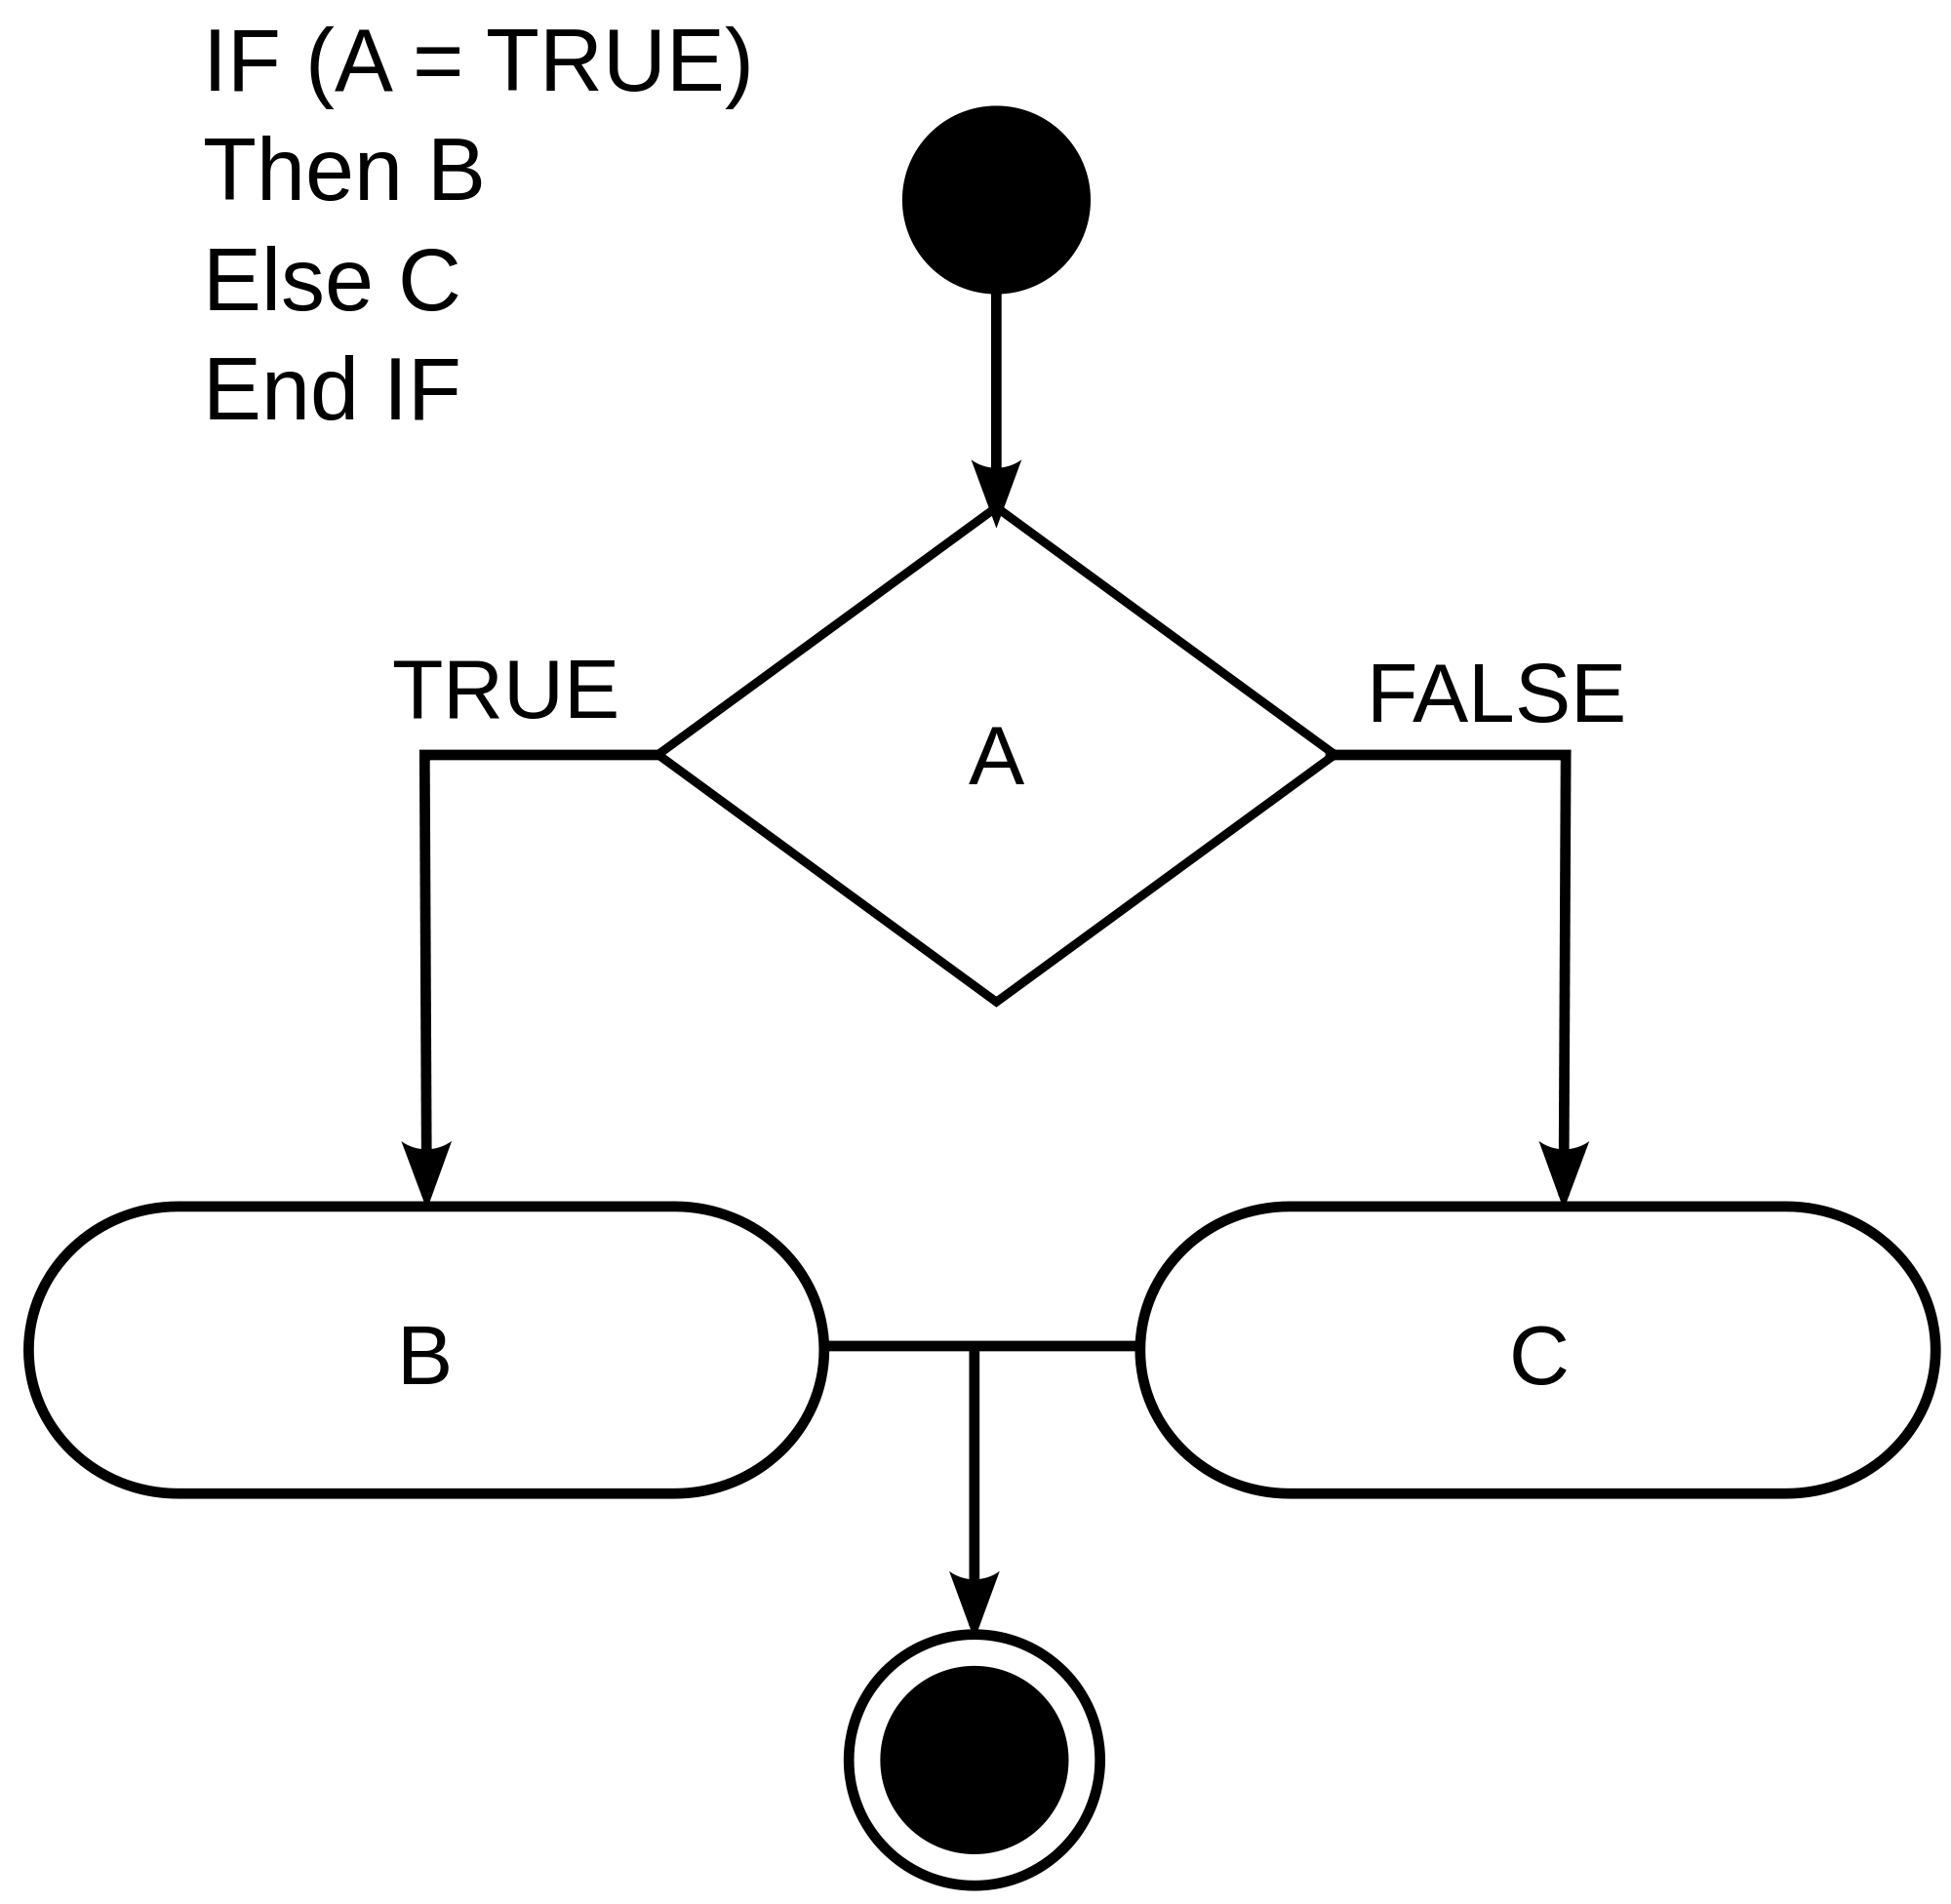
\includegraphics{figure/ifelse.png}

\texttt{if}與\texttt{else}下方的程式碼必須要使用\texttt{\{\}}將程式碼包起來,若程式碼只有一行,可省略\texttt{\{\}},但為閱讀方便,建議不要省略\texttt{\{\}}。

舉例來說,若考試分數\textbf{大於等於60分},則印出\textbf{及格}字樣,小於60分則印出\textbf{不及格}字樣,程式範例如下:

\begin{Shaded}
\begin{Highlighting}[]
\NormalTok{score<-}\DecValTok{59}
\NormalTok{if(score>=}\DecValTok{60}\NormalTok{)\{}
  \KeywordTok{print}\NormalTok{(}\StringTok{"及格"}\NormalTok{)}
\NormalTok{\}else\{}
  \KeywordTok{print}\NormalTok{(}\StringTok{"不及格"}\NormalTok{)}
\NormalTok{\}}
\end{Highlighting}
\end{Shaded}

\begin{verbatim}
## [1] "不及格"
\end{verbatim}

\begin{Shaded}
\begin{Highlighting}[]
\NormalTok{score<-}\DecValTok{80}
\NormalTok{if(score>=}\DecValTok{60}\NormalTok{)\{}
  \KeywordTok{print}\NormalTok{(}\StringTok{"及格"}\NormalTok{)}
\NormalTok{\}else\{}
  \KeywordTok{print}\NormalTok{(}\StringTok{"不及格"}\NormalTok{)}
\NormalTok{\}}
\end{Highlighting}
\end{Shaded}

\begin{verbatim}
## [1] "及格"
\end{verbatim}

\subsection{if-else if-else}\label{if-else-if-else}

很多時候必須要使用多重邏輯判斷,若考試分數大於等於90分,印出\textbf{優良},介於60到90分間,印出\textbf{及格},小於60分則印出\textbf{不及格},此時就會用到多重邏輯,使用多重邏輯時,會在\texttt{if}和\texttt{else}間新增邏輯區段\textbf{else
if},程式範例如下:

\begin{Shaded}
\begin{Highlighting}[]
\NormalTok{score<-}\DecValTok{95}
\NormalTok{if(score>=}\DecValTok{90}\NormalTok{)\{}
  \KeywordTok{print}\NormalTok{(}\StringTok{"優秀"}\NormalTok{)}
\NormalTok{\}else if(score>=}\DecValTok{60}\NormalTok{)\{}
  \KeywordTok{print}\NormalTok{(}\StringTok{"及格"}\NormalTok{)}
\NormalTok{\}else\{}
  \KeywordTok{print}\NormalTok{(}\StringTok{"不及格"}\NormalTok{)}
\NormalTok{\}}
\end{Highlighting}
\end{Shaded}

\begin{verbatim}
## [1] "優秀"
\end{verbatim}

\texttt{if-else\ if-else}敘述是有順序的,若在\texttt{if}敘述判斷為真,就算後方\texttt{else\ if}判斷也為真,也只會執行\texttt{if}區段的程式碼,如上述範例,95分大於等於90分(if邏輯),也大於等於60分(else
if邏輯),但最後只印出\textbf{優秀}字樣。

\subsection{巢狀if}\label{if}

巢狀if是指在\texttt{if}區段程式碼內包含其他\texttt{if-else}判斷,舉例來說,若國文分數與英文分數皆大於等於60分,印出\textbf{全部及格},國文分數大於等於60分,英文小於60分,則印\textbf{國文及格,英文再加油},以此類推,程式範例如下:

\begin{Shaded}
\begin{Highlighting}[]
\NormalTok{CHscore<-}\DecValTok{95} \NormalTok{##國文成績}
\NormalTok{ENscore<-}\DecValTok{55} \NormalTok{##英文成績}
\NormalTok{if(CHscore>=}\DecValTok{60}\NormalTok{)\{}
  \NormalTok{if(ENscore>=}\DecValTok{60}\NormalTok{)\{}
    \KeywordTok{print}\NormalTok{(}\StringTok{"全部及格"}\NormalTok{)}
  \NormalTok{\}else\{}
    \KeywordTok{print}\NormalTok{(}\StringTok{"國文及格,英文再加油"}\NormalTok{)}
  \NormalTok{\}}
\NormalTok{\}else\{}
  \NormalTok{if(ENscore>=}\DecValTok{60}\NormalTok{)\{}
    \KeywordTok{print}\NormalTok{(}\StringTok{"英文及格,國文再加油"}\NormalTok{)}
  \NormalTok{\}else\{}
    \KeywordTok{print}\NormalTok{(}\StringTok{"全部不及格"}\NormalTok{)}
  \NormalTok{\}}
\NormalTok{\}}
\end{Highlighting}
\end{Shaded}

\begin{verbatim}
## [1] "國文及格,英文再加油"
\end{verbatim}

\subsection{ifelse()}\label{ifelse}

\texttt{ifelse()}函數可用最短的方式取代\texttt{if-else}敘述,使用方法為\texttt{ifelse(邏輯判斷,判斷為真要執行的程式碼,判斷為偽要執行的程式碼)},依上述範例,重寫程式碼如下:

\begin{Shaded}
\begin{Highlighting}[]
\NormalTok{score<-}\DecValTok{80}
\KeywordTok{ifelse}\NormalTok{(score>=}\DecValTok{60}\NormalTok{,}\StringTok{"及格"}\NormalTok{,}\StringTok{"不及格"}\NormalTok{)}
\end{Highlighting}
\end{Shaded}

\begin{verbatim}
## [1] "及格"
\end{verbatim}

值得注意的是,\texttt{ifelse()}可判斷向量,也就是可一次\textbf{判斷多個元素}

\begin{Shaded}
\begin{Highlighting}[]
\NormalTok{scoreVector<-}\KeywordTok{c}\NormalTok{(}\DecValTok{30}\NormalTok{,}\DecValTok{90}\NormalTok{,}\DecValTok{50}\NormalTok{,}\DecValTok{60}\NormalTok{,}\DecValTok{80}\NormalTok{)}
\KeywordTok{ifelse}\NormalTok{(scoreVector>=}\DecValTok{60}\NormalTok{,}\StringTok{"及格"}\NormalTok{, }\StringTok{"不及格"}\NormalTok{)}
\end{Highlighting}
\end{Shaded}

\begin{verbatim}
## [1] "不及格" "及格"   "不及格" "及格"   "及格"
\end{verbatim}

\section{迴圈}

\subsection{for}\label{for}

R語言的\texttt{for}迴圈寫法和其他語言不同,首先必須建立需要逐一執行的參數向量或序列,再使用\texttt{for}迴圈逐一執行,程式寫法為\texttt{for\ (單一變數\ in\ 參數向量)\{\ 程式碼\ \}},範例如下:

\begin{Shaded}
\begin{Highlighting}[]
\NormalTok{for (n in }\DecValTok{1}\NormalTok{:}\DecValTok{10}\NormalTok{)\{ }\CommentTok{#n為單一變數,1:10為需要逐一執行的參數向量}
  \KeywordTok{print}\NormalTok{(n)}
\NormalTok{\}}
\end{Highlighting}
\end{Shaded}

\begin{verbatim}
## [1] 1
## [1] 2
## [1] 3
## [1] 4
## [1] 5
## [1] 6
## [1] 7
## [1] 8
## [1] 9
## [1] 10
\end{verbatim}

\texttt{for}迴圈也可和\texttt{if-else}函數合併使用,如:

\begin{Shaded}
\begin{Highlighting}[]
\NormalTok{for (n in }\DecValTok{1}\NormalTok{:}\DecValTok{10}\NormalTok{)\{}
  \NormalTok{if(n%%}\DecValTok{2}\NormalTok{==}\DecValTok{0}\NormalTok{)\{ }\CommentTok{#偶數直接輸出數字}
    \KeywordTok{print}\NormalTok{(n)}
  \NormalTok{\}else\{}
    \KeywordTok{print}\NormalTok{(}\StringTok{"奇數"}\NormalTok{) }\CommentTok{#奇數則輸出"奇數"}
  \NormalTok{\}}
\NormalTok{\}}
\end{Highlighting}
\end{Shaded}

\begin{verbatim}
## [1] "奇數"
## [1] 2
## [1] "奇數"
## [1] 4
## [1] "奇數"
## [1] 6
## [1] "奇數"
## [1] 8
## [1] "奇數"
## [1] 10
\end{verbatim}

\subsection{while}\label{while}

\texttt{while}函數則是在每次執行迴圈時檢查while邏輯判斷是否為真,若邏輯判斷為真,就會執行區段程式碼,若邏輯判斷為偽,則會結束迴圈執行。

\begin{Shaded}
\begin{Highlighting}[]
\NormalTok{x<-}\DecValTok{0}
\NormalTok{while(x<=}\DecValTok{5}\NormalTok{)\{}
  \KeywordTok{print}\NormalTok{(x)}
  \NormalTok{x<-x}\DecValTok{+1}
\NormalTok{\}}
\end{Highlighting}
\end{Shaded}

\begin{verbatim}
## [1] 0
## [1] 1
## [1] 2
## [1] 3
## [1] 4
## [1] 5
\end{verbatim}

\subsection{break}\label{break}

若遇特殊情形想\textbf{結束}迴圈執行,可使用\texttt{break}指令

\begin{Shaded}
\begin{Highlighting}[]
\NormalTok{for(n in }\DecValTok{1}\NormalTok{:}\DecValTok{10}\NormalTok{)\{}
  \NormalTok{if(n==}\DecValTok{5}\NormalTok{)\{}
    \NormalTok{break ##一執行到5,跳出迴圈,不再執行之後的迴圈}
  \NormalTok{\}}
  \KeywordTok{print}\NormalTok{(n)}
\NormalTok{\}}
\end{Highlighting}
\end{Shaded}

\begin{verbatim}
## [1] 1
## [1] 2
## [1] 3
## [1] 4
\end{verbatim}

\subsection{next}\label{next}

若遇特殊情形想\textbf{跳過}迴圈執行,可使用\texttt{next}指令

\begin{Shaded}
\begin{Highlighting}[]
\NormalTok{for(n in }\DecValTok{1}\NormalTok{:}\DecValTok{10}\NormalTok{)\{}
  \NormalTok{if(n==}\DecValTok{5}\NormalTok{)\{}
    \NormalTok{next ##跳過5,直接執行下一個迴圈}
  \NormalTok{\}}
  \KeywordTok{print}\NormalTok{(n)}
\NormalTok{\}}
\end{Highlighting}
\end{Shaded}

\begin{verbatim}
## [1] 1
## [1] 2
## [1] 3
## [1] 4
## [1] 6
## [1] 7
## [1] 8
## [1] 9
## [1] 10
\end{verbatim}

\chapter{探索式資料分析}\label{eda}

You can label chapter and section titles using \texttt{\{\#label\}}
after them, e.g., we can reference Chapter \ref{intro}. If you do not
manually label them, there will be automatic labels anyway, e.g.,
Chapter \ref{methods}.

Figures and tables with captions will be placed in \texttt{figure} and
\texttt{table} environments, respectively.

\begin{Shaded}
\begin{Highlighting}[]
\KeywordTok{par}\NormalTok{(}\DataTypeTok{mar =} \KeywordTok{c}\NormalTok{(}\DecValTok{4}\NormalTok{, }\DecValTok{4}\NormalTok{, .}\DecValTok{1}\NormalTok{, .}\DecValTok{1}\NormalTok{))}
\KeywordTok{plot}\NormalTok{(pressure, }\DataTypeTok{type =} \StringTok{'b'}\NormalTok{, }\DataTypeTok{pch =} \DecValTok{19}\NormalTok{)}
\end{Highlighting}
\end{Shaded}

\begin{figure}

{\centering 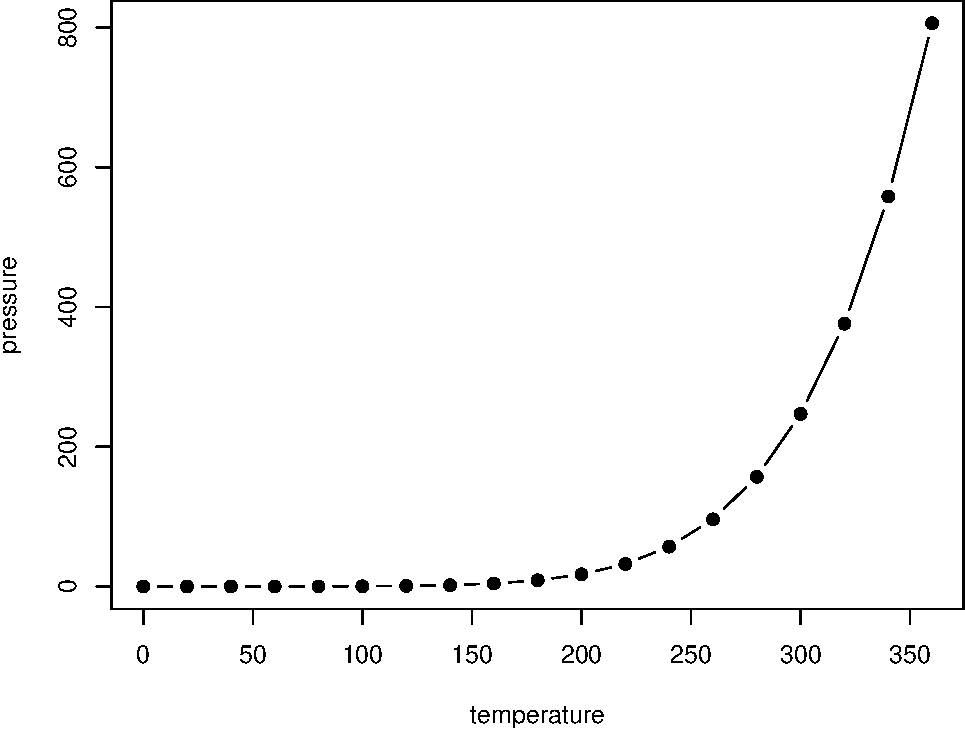
\includegraphics[width=0.8\linewidth]{DataAnalyticsWithR_files/figure-latex/nice-fig6-1} 

}

\caption{Here is a nice figure!}\label{fig:nice-fig6}
\end{figure}

Reference a figure by its code chunk label with the \texttt{fig:}
prefix, e.g., see Figure \ref{fig:nice-fig}. Similarly, you can
reference tables generated from \texttt{knitr::kable()}, e.g., see Table
\ref{tab:nice-tab}.

\begin{Shaded}
\begin{Highlighting}[]
\NormalTok{knitr::}\KeywordTok{kable}\NormalTok{(}
  \KeywordTok{head}\NormalTok{(iris, }\DecValTok{20}\NormalTok{), }\DataTypeTok{caption =} \StringTok{'Here is a nice table!'}\NormalTok{,}
  \DataTypeTok{booktabs =} \OtherTok{TRUE}
\NormalTok{)}
\end{Highlighting}
\end{Shaded}

\begin{table}

\caption{\label{tab:nice-tab6}Here is a nice table!}
\centering
\begin{tabular}[t]{rrrrl}
\toprule
Sepal.Length & Sepal.Width & Petal.Length & Petal.Width & Species\\
\midrule
5.1 & 3.5 & 1.4 & 0.2 & setosa\\
4.9 & 3.0 & 1.4 & 0.2 & setosa\\
4.7 & 3.2 & 1.3 & 0.2 & setosa\\
4.6 & 3.1 & 1.5 & 0.2 & setosa\\
5.0 & 3.6 & 1.4 & 0.2 & setosa\\
\addlinespace
5.4 & 3.9 & 1.7 & 0.4 & setosa\\
4.6 & 3.4 & 1.4 & 0.3 & setosa\\
5.0 & 3.4 & 1.5 & 0.2 & setosa\\
4.4 & 2.9 & 1.4 & 0.2 & setosa\\
4.9 & 3.1 & 1.5 & 0.1 & setosa\\
\addlinespace
5.4 & 3.7 & 1.5 & 0.2 & setosa\\
4.8 & 3.4 & 1.6 & 0.2 & setosa\\
4.8 & 3.0 & 1.4 & 0.1 & setosa\\
4.3 & 3.0 & 1.1 & 0.1 & setosa\\
5.8 & 4.0 & 1.2 & 0.2 & setosa\\
\addlinespace
5.7 & 4.4 & 1.5 & 0.4 & setosa\\
5.4 & 3.9 & 1.3 & 0.4 & setosa\\
5.1 & 3.5 & 1.4 & 0.3 & setosa\\
5.7 & 3.8 & 1.7 & 0.3 & setosa\\
5.1 & 3.8 & 1.5 & 0.3 & setosa\\
\bottomrule
\end{tabular}
\end{table}

You can write citations, too. For example, we are using the
\textbf{bookdown} package \citep{R-bookdown} in this sample book, which
was built on top of R Markdown and \textbf{knitr} \citep{xie2015}.

\chapter{資料視覺化}\label{vis}

You can label chapter and section titles using \texttt{\{\#label\}}
after them, e.g., we can reference Chapter \ref{intro}. If you do not
manually label them, there will be automatic labels anyway, e.g.,
Chapter \ref{methods}.

Figures and tables with captions will be placed in \texttt{figure} and
\texttt{table} environments, respectively.

\begin{Shaded}
\begin{Highlighting}[]
\KeywordTok{par}\NormalTok{(}\DataTypeTok{mar =} \KeywordTok{c}\NormalTok{(}\DecValTok{4}\NormalTok{, }\DecValTok{4}\NormalTok{, .}\DecValTok{1}\NormalTok{, .}\DecValTok{1}\NormalTok{))}
\KeywordTok{plot}\NormalTok{(pressure, }\DataTypeTok{type =} \StringTok{'b'}\NormalTok{, }\DataTypeTok{pch =} \DecValTok{19}\NormalTok{)}
\end{Highlighting}
\end{Shaded}

\begin{figure}

{\centering 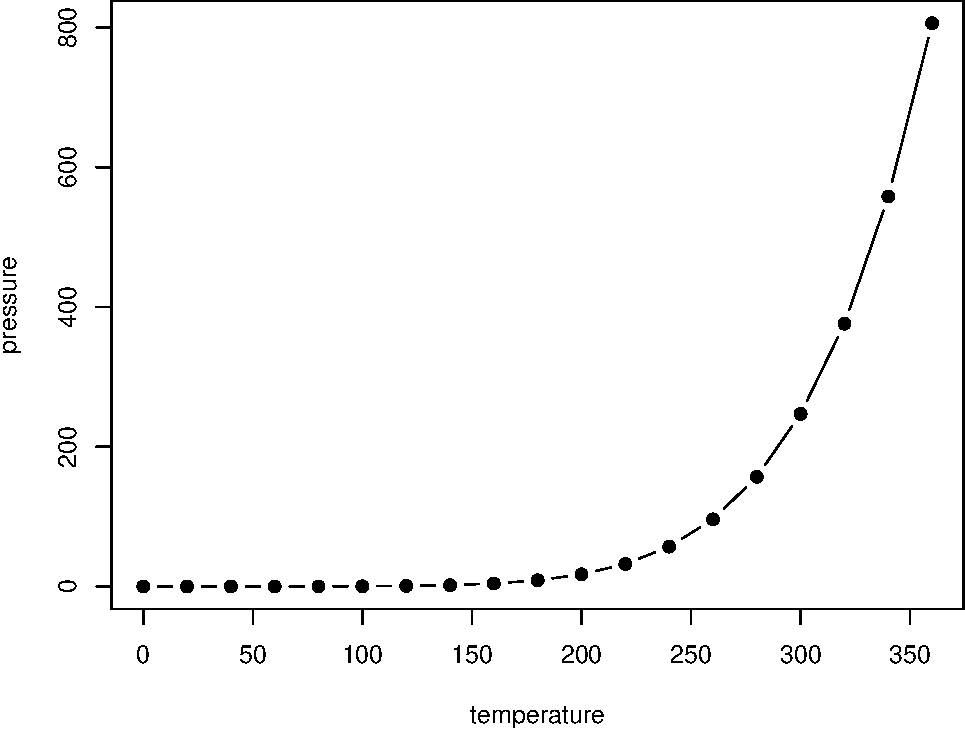
\includegraphics[width=0.8\linewidth]{DataAnalyticsWithR_files/figure-latex/nice-fig7-1} 

}

\caption{Here is a nice figure!}\label{fig:nice-fig7}
\end{figure}

Reference a figure by its code chunk label with the \texttt{fig:}
prefix, e.g., see Figure \ref{fig:nice-fig}. Similarly, you can
reference tables generated from \texttt{knitr::kable()}, e.g., see Table
\ref{tab:nice-tab}.

\begin{Shaded}
\begin{Highlighting}[]
\NormalTok{knitr::}\KeywordTok{kable}\NormalTok{(}
  \KeywordTok{head}\NormalTok{(iris, }\DecValTok{20}\NormalTok{), }\DataTypeTok{caption =} \StringTok{'Here is a nice table!'}\NormalTok{,}
  \DataTypeTok{booktabs =} \OtherTok{TRUE}
\NormalTok{)}
\end{Highlighting}
\end{Shaded}

\begin{table}

\caption{\label{tab:nice-tab7}Here is a nice table!}
\centering
\begin{tabular}[t]{rrrrl}
\toprule
Sepal.Length & Sepal.Width & Petal.Length & Petal.Width & Species\\
\midrule
5.1 & 3.5 & 1.4 & 0.2 & setosa\\
4.9 & 3.0 & 1.4 & 0.2 & setosa\\
4.7 & 3.2 & 1.3 & 0.2 & setosa\\
4.6 & 3.1 & 1.5 & 0.2 & setosa\\
5.0 & 3.6 & 1.4 & 0.2 & setosa\\
\addlinespace
5.4 & 3.9 & 1.7 & 0.4 & setosa\\
4.6 & 3.4 & 1.4 & 0.3 & setosa\\
5.0 & 3.4 & 1.5 & 0.2 & setosa\\
4.4 & 2.9 & 1.4 & 0.2 & setosa\\
4.9 & 3.1 & 1.5 & 0.1 & setosa\\
\addlinespace
5.4 & 3.7 & 1.5 & 0.2 & setosa\\
4.8 & 3.4 & 1.6 & 0.2 & setosa\\
4.8 & 3.0 & 1.4 & 0.1 & setosa\\
4.3 & 3.0 & 1.1 & 0.1 & setosa\\
5.8 & 4.0 & 1.2 & 0.2 & setosa\\
\addlinespace
5.7 & 4.4 & 1.5 & 0.4 & setosa\\
5.4 & 3.9 & 1.3 & 0.4 & setosa\\
5.1 & 3.5 & 1.4 & 0.3 & setosa\\
5.7 & 3.8 & 1.7 & 0.3 & setosa\\
5.1 & 3.8 & 1.5 & 0.3 & setosa\\
\bottomrule
\end{tabular}
\end{table}

You can write citations, too. For example, we are using the
\textbf{bookdown} package \citep{R-bookdown} in this sample book, which
was built on top of R Markdown and \textbf{knitr} \citep{xie2015}.

\chapter{從小數據到大數據分析}\label{big}

\section{R + Hadoop}\label{r-hadoop}

\section{RHadoop安裝測試流程 (Cloudera)}\label{rhadoop-cloudera}

安裝與測試日期2016/05/12

\subsection{系統/軟體版本資訊}

\begin{itemize}
\tightlist
\item
  Cloudera Hadoop Platform: CDH-5.4.5
  \href{http://www.cloudera.com/downloads/cdh/5-4-5.html}{下載}
\item
  R for Linux 3.3.0
  \href{https://cran.rstudio.com/bin/linux/redhat/README}{安裝說明}
\item
  RStudio Server
  \href{https://www.rstudio.com/products/rstudio/download-server/}{下載}
\item
  RHadoop (latest version on May 12, 2016)
  \href{https://github.com/RevolutionAnalytics/RHadoop/wiki/Downloads}{下載}

  \begin{itemize}
  \tightlist
  \item
    ravro-1.0.3
  \item
    plyrmr-0.6.0
  \item
    rmr-3.3.1
  \item
    rhdfs-1.0.8
  \item
    rhbase-1.2.1
  \end{itemize}
\end{itemize}

\subsection{參考資料}

\begin{itemize}
\tightlist
\item
  \href{https://github.com/RevolutionAnalytics/RHadoop/wiki/Installing-RHadoop-on-RHEL}{RHadoop安裝說明文件}
\item
  \href{https://bigdatastudy.hackpad.com/ep/pad/static/IADMBeqF0vV}{RHadoop安裝步驟}
\item
  \href{http://unix.stackexchange.com/questions/271514/setting-persistent-environment-variable-in-centos-7-issue}{Setting
  persistent environment variable in CentOS 7 issue}
\item
  \href{https://community.cloudera.com/t5/CDH-Manual-Installation/How-to-resolve-quot-Permission-denied-quot-errors-in-CDH/ta-p/36141}{How
  to resolve ``Permission denied'' errors in CDH}
\end{itemize}

\subsection{安裝步驟}

\begin{enumerate}
\def\labelenumi{\arabic{enumi}.}
\tightlist
\item
  下載Cloudera CDH QuickStart VM
  \href{http://www.cloudera.com/developers/get-started-with-hadoop-tutorial.html}{Cloudera
  VM}
\item
  安裝R
  \href{https://cran.rstudio.com/bin/linux/redhat/README}{安裝說明}
\item
  安裝RHadoop
  \href{https://bigdatastudy.hackpad.com/ep/pad/static/IADMBeqF0vV}{RHadoop安裝步驟}
\item
  安裝RStudio Server
  \href{https://www.rstudio.com/products/rstudio/download-server/}{說明}
\end{enumerate}

\subsubsection{Cloudera CDH QuickStart
VM}\label{cloudera-cdh-quickstart-vm}

Cloudera CDH QuickStart
VM是由Cloudera提供的虛擬機器,內涵Linux系統與預載多項Hadoop相關服務,適合想了解Hadoop運作的初學者。

下載VM後,用Virtural Box 開啟即可。

\begin{itemize}
\tightlist
\item
  \href{http://www.cloudera.com/developers/get-started-with-hadoop-tutorial.html}{Cloudera
  CDH QuickStart VM下載處}
\item
  \href{https://www.virtualbox.org/}{Virtural Box下載處}
\end{itemize}

以下安裝步驟都在Cloudera CDH QuickStart VM內進行

\subsubsection{安裝R}\label{r}

\begin{itemize}
\tightlist
\item
  Cloudera CDH用的Linux作業系統是CentOS
\item
  依照安裝說明,需要先安裝Extra Packages for Enterprise Linux
  (EPEL),但系統內有預載,所以可以不用按照說明重新下載安裝,直接執行\texttt{sudo\ yum\ install\ epel-release}指令即可
\item
  步驟:安裝最新EPRL,更新yum,安裝R。打開Terminal輸入以下指令。
\end{itemize}

\begin{verbatim}
sudo yum install epel-release
sudo yum update
sudo yum install R
\end{verbatim}

\subsubsection{安裝RHadoop-1 先進行環境設定}\label{rhadoop-1-}

設定\texttt{HADOOP\_CMD}與\texttt{HADOOP\_STREAMING}兩項環境參數,路徑可能會不同(尤其是\texttt{HADOOP\_STREAMING})

\begin{enumerate}
\def\labelenumi{\arabic{enumi}.}
\item
  尋找\texttt{HADOOP\_STREAMING}路徑方法

\begin{verbatim}
find / -name hadoop-streaming-*.jar
\end{verbatim}
\item
  設定\texttt{HADOOP\_CMD}與\texttt{HADOOP\_STREAMING}兩項環境參數,路徑記得換成自己的

\begin{verbatim}
echo export HADOOP_CMD="/usr/bin/hadoop">/etc/profile.d/hadoopenv.sh
echo export HADOOP_STREAMING=
"/opt/cloudera/parcels/CDH-5.4.5-1.cdh5.4.5.p0.7/lib/hadoop-mapreduce/
    hadoop-streaming-2.6.0-cdh5.4.5.jar" > /etc/profile.d/hadoopenv.sh
chmod 0755 /etc/profile.d/hadoopenv.sh
\end{verbatim}
\end{enumerate}

\subsubsection{安裝RHadoop-2 rmr2}\label{rhadoop-2-rmr2}

\begin{itemize}
\tightlist
\item
  每個Node都要裝
\item
  安裝前先至\href{https://github.com/RevolutionAnalytics/rmr2/blob/master/pkg/DESCRIPTION}{說明檔}看需要先安裝哪些其他的packages,Depends
  和 Imports 所列的packages都要裝
\item
  以下為安裝packages的程式碼,在R內執行(在Terminal輸入\texttt{R},就能進入R軟體)
\end{itemize}

\begin{Shaded}
\begin{Highlighting}[]
\KeywordTok{install.packages}\NormalTok{(}\KeywordTok{c}\NormalTok{(}\StringTok{"methods"}\NormalTok{,}\StringTok{"Rcpp"}\NormalTok{, }\StringTok{"RJSONIO"}\NormalTok{, }\StringTok{"digest"}\NormalTok{, }\StringTok{"functional"}\NormalTok{, }
                   \StringTok{"reshape2"}\NormalTok{,}\StringTok{"stringr"}\NormalTok{, }\StringTok{"plyr"}\NormalTok{, }\StringTok{"caTools"}\NormalTok{,}\StringTok{"quickcheck"}\NormalTok{,}\StringTok{"testthat"}\NormalTok{), }
                 \DataTypeTok{dependencies=}\OtherTok{TRUE}\NormalTok{, }\DataTypeTok{repos=}\StringTok{'http://cran.rstudio.com/'}\NormalTok{)}
\end{Highlighting}
\end{Shaded}

\begin{itemize}
\tightlist
\item
  使用\texttt{q()}指令,跳出R軟體
\item
  \href{https://github.com/RevolutionAnalytics/RHadoop/wiki/Downloads}{下載rmr2}
\item
  安裝(請將\texttt{rmr2\_2.3.0.tar.gz}替換成剛剛下載的安裝檔路徑)
\end{itemize}

\begin{verbatim}
sudo R CMD INSTALL rmr2_2.3.0.tar.gz
\end{verbatim}

\subsubsection{安裝RHadoop-3 rhdfs}\label{rhadoop-3-rhdfs}

\begin{itemize}
\tightlist
\item
  只要裝在會跑R的那個Node
\item
  在裝之前,先Check是否有安裝JDK (測試JDK 1.8.0\_91沒問題)
\item
  Check環境變數JAVA\_HOME是否有設好
\end{itemize}

\begin{verbatim}
echo $JAVA_HOME
\end{verbatim}

若什麼都沒有回傳,先設定環境變數(將\texttt{/usr/java/jdk1.8.0\_91}換成自己的路徑)

\begin{verbatim}
echo export JAVA_HOME="/usr/java/jdk1.8.0_91">/etc/profile.d/jdkenv.sh
\end{verbatim}

為了讓R可以跑JAVA,在Terminal輸入

\begin{verbatim}
R CMD javareconf
\end{verbatim}

然後進到R程式(在Terminal輸入\texttt{R},就能進入R軟體),安裝\texttt{rJava}
package

\begin{Shaded}
\begin{Highlighting}[]
\KeywordTok{install.packages}\NormalTok{(}\StringTok{"rJava"}\NormalTok{,}\DataTypeTok{dependencies=}\OtherTok{TRUE}\NormalTok{, }\DataTypeTok{repos=}\StringTok{'http://cran.rstudio.com/'}\NormalTok{)}
\end{Highlighting}
\end{Shaded}

最後跳出R程式,\href{https://github.com/RevolutionAnalytics/RHadoop/wiki/Downloads}{下載rhdfs},安裝rhdfs

\begin{itemize}
\tightlist
\item
  將\texttt{/usr/bin/hadoop}換成自己的\texttt{HADOOP\_CMD}路徑
\item
  \texttt{rhdfs\_1.0.8.tar.gz}換成下載的安裝檔路徑)
\end{itemize}

\begin{verbatim}
sudo HADOOP_CMD=/usr/bin/hadoop R CMD INSTALL rhdfs_1.0.8.tar.gz
\end{verbatim}

\subsection{測試前,先解決權限問題}

\begin{itemize}
\tightlist
\item
  預設hdfs的存取權限不足,所以要打開
\item
  將\texttt{user01}改為自己的使用者名稱
\end{itemize}

\begin{verbatim}
sudo -u hdfs hadoop fs -mkdir /user/user01
sudo -u hdfs hadoop fs -chown user01 /user/user01
\end{verbatim}

\subsection{測試}

進入R測試以下程式碼是否能執行

\begin{Shaded}
\begin{Highlighting}[]
\KeywordTok{Sys.setenv}\NormalTok{(}\DataTypeTok{HADOOP_CMD=}\StringTok{"/usr/bin/hadoop"}\NormalTok{)}
\KeywordTok{Sys.setenv}\NormalTok{(}\DataTypeTok{HADOOP_STREAMING=}\StringTok{"/opt/cloudera/parcels/CDH-5.4.5-1.cdh5.4.5.p0.7/lib/hadoop-mapreduce/hadoop-streaming-2.6.0-cdh5.4.5.jar"}\NormalTok{)}
\KeywordTok{library}\NormalTok{(rmr2)}
\CommentTok{#test mapreduce}
\NormalTok{small.ints =}\StringTok{ }\KeywordTok{to.dfs}\NormalTok{(}\DecValTok{1}\NormalTok{:}\DecValTok{100}\NormalTok{)}
\NormalTok{out<-}\KeywordTok{mapreduce}\NormalTok{(}
    \DataTypeTok{input =} \NormalTok{small.ints, }
    \DataTypeTok{map =} \NormalTok{function(., v) }\KeywordTok{cbind}\NormalTok{(v, v^}\DecValTok{2}\NormalTok{))}
\KeywordTok{head}\NormalTok{(}\KeywordTok{from.dfs}\NormalTok{(out))}
\end{Highlighting}
\end{Shaded}

\subsection{安裝RStudio Server}\label{rstudio-server}

\href{https://www.rstudio.com/products/rstudio/download-server/}{官方下載與安裝說明}

在Terminal執行以下程式碼

\begin{itemize}
\tightlist
\item
  檔案連結\texttt{https://download2.rstudio.org/rstudio-server-rhel-0.99.896-x86\_64.rpm}可能有最新版,請Check\href{https://www.rstudio.com/products/rstudio/download-server/}{官網}
\end{itemize}

\begin{verbatim}
wget https://download2.rstudio.org/rstudio-server-rhel-0.99.896-x86_64.rpm
sudo yum install --nogpgcheck rstudio-server-rhel-0.99.896-x86_64.rpm
\end{verbatim}

打開瀏覽器,輸入\texttt{http://localhost:8787/},就能進入RStudio
Server了!

測完收工~

\section{RHadoop MapReduce: easy word
count}\label{rhadoop-mapreduce-easy-word-count}

\begin{Shaded}
\begin{Highlighting}[]
\NormalTok{Debate<-}\KeywordTok{readLines}\NormalTok{(}\StringTok{"https://raw.githubusercontent.com/yijutseng/BigDataCGUIM/master/RepDebateMiami.txt"}\NormalTok{)}
\NormalTok{DebateSplit<-}\KeywordTok{unlist}\NormalTok{(}\KeywordTok{strsplit}\NormalTok{(}\KeywordTok{tolower}\NormalTok{(Debate),}\DataTypeTok{split =} \StringTok{' |}\CharTok{\textbackslash{}\textbackslash{}}\StringTok{.|}\CharTok{\textbackslash{}\textbackslash{}}\StringTok{,|}\CharTok{\textbackslash{}\textbackslash{}}\StringTok{?'}\NormalTok{))}
\CommentTok{#table(DebateSplit)}
\end{Highlighting}
\end{Shaded}

\begin{Shaded}
\begin{Highlighting}[]
\NormalTok{DebateSplitDFS =}\StringTok{ }\KeywordTok{to.dfs}\NormalTok{(DebateSplit)}
\NormalTok{result =}\StringTok{ }\KeywordTok{mapreduce}\NormalTok{(}
    \DataTypeTok{input =} \NormalTok{DebateSplitDFS,}
    \DataTypeTok{map =} \NormalTok{function(.,v) }\KeywordTok{keyval}\NormalTok{(v, }\DecValTok{1}\NormalTok{),}
    \DataTypeTok{reduce =} \NormalTok{function(k,vv) }\KeywordTok{keyval}\NormalTok{(k, }\KeywordTok{sum}\NormalTok{(vv)))}
\KeywordTok{head}\NormalTok{(result)}
\end{Highlighting}
\end{Shaded}

\section{R + Spark}\label{r-spark}

\chapter*{作者資訊}\label{author}
\addcontentsline{toc}{chapter}{作者資訊}

曾意儒 Yi-Ju Tseng

\href{http://im.cgu.edu.tw/bin/home.php}{長庚大學 資訊管理學系} 助理教授

\href{http://yijutseng.github.io}{個人網站}

\href{http://yijutseng.github.io/Lab/}{數位健康實驗室}

\bibliography{packages,book}


\end{document}
